\section{Experiments}
\label{sec:experiments}

We test the claims of Sections~\ref{sec:analysis} and~\ref{sec:method} in the order in which they were
made: FCT improves all three networks over their own baselines, most on
unseen data (Section~\ref{sec:main}), and a label-aware variant generalizes to six more centres
(Section~\ref{sec:polypgen}); FCT makes predictions more flip-consistent
(Section~\ref{sec:flip}); a per-image analysis shows where its gains come from
(Section~\ref{sec:where}); and a study of the loss terms shows that the multi-view supervision gives
most of the gain, while the label-aware weights shape the gradient as Corollary~\ref{cor:lag} predicts and
need no tuning (Section~\ref{sec:ablation}).
Section~\ref{sec:cost} reports its cost.

\subsection{Datasets and Evaluation Protocol}
\label{sec:setup}

We train on 1,288 images, 800 from Kvasir-SEG~\cite{jha2020kvasir} and 488 from
CVC-ClinicDB~\cite{bernal2015clinicdb}, drawn from the 1,450-image training split
of~\cite{fan2020pranet}; none of them appears in a test set. Because this set is smaller than the full
split, absolute scores are not directly comparable with published ones, and every comparison below is
between models trained on the same images. We test on the five standard test sets: the test splits of
Kvasir-SEG (100 images) and CVC-ClinicDB (62), which we call seen, and
CVC-ColonDB~\cite{tajbakhsh2016colondb} (380), CVC-300~\cite{vazquez2017endoscene} (60) and
ETIS~\cite{silva2014etis} (196), which are unseen in training. CVC-ColonDB and CVC-300 come from the same
group as CVC-ClinicDB, whereas ETIS comes from another centre.

We report the mean Dice (mDice) of the evaluation toolbox of~\cite{fan2020pranet}, which Polyp-PVT also
uses: each predicted map is min-max normalized and binarized at 256 thresholds, and the Dice coefficient
is averaged over images and thresholds. The flip gap of Eq.~\eqref{eq:flipgap} is computed on the masks
thresholded at 0.5 at the input resolution of the network, with add-one smoothing so that two empty
masks agree. Each network is evaluated on the five test sets after every epoch with the per-image Dice
of the official Polyp-PVT code, and we keep the epoch with the highest five-set mean, for vanilla and
FCT alike; Section~\ref{sec:main} also reports the gains without this selection.

Each configuration is trained with six random seeds, and vanilla and FCT share each seed. We report
the mean and standard deviation (SD) over seeds, the mean paired difference with its 95\% confidence
interval (CI) from the $t$-distribution with five degrees of freedom, and the number of seeds on which
FCT scores higher. An exact permutation test over all 924 ways of splitting the twelve runs of a
comparison into two groups of six reaches the same conclusion as the CI for every entry of
Tables~\ref{tab:main_polyppvt} and~\ref{tab:main_pranetv2}.

\subsection{Implementation Details}
\label{sec:implementation}

We add FCT to three networks without changing their architectures or retuning their recipes.
Polyp-PVT~\cite{dong2023polyppvt} uses a PVTv2-B2 encoder~\cite{wang2022pvtv2}. As in its official code,
it is trained with AdamW, a learning rate of $10^{-4}$, a weight decay of $10^{-4}$, batches of 16 images
of $352\times352$ pixels, input scales of 0.75, 1 and 1.25, element-wise gradient clipping at 0.5 and 99 epochs, and
its encoder has a stochastic-depth rate of 0.1; we add mixed precision. Its official recipe applies no orientation
augmentation by default, and we keep this default, so vanilla Polyp-PVT never sees a flipped image.
PraNet-V2~\cite{hu2026pranetv2} uses a Res2Net-50 encoder~\cite{gao2021res2net}, which has no stochastic
depth, and is trained with Adam, a constant learning rate of $10^{-4}$, batches of 8 images and 29
epochs, with the data pipeline, input scales and mixed precision of Polyp-PVT. ASGNet~\cite{sun2026asgnet} uses a PVTv2-B3 encoder and keeps its own
recipe: Adam, batches of 40 images accumulated over eight parts, 79 epochs at a single scale in full
precision, a cosine learning-rate schedule, and its own data loader, which applies random horizontal
flips, crops, rotations, colour changes and label noise. Unlike the other two, ASGNet is therefore
trained with flip augmentation even without FCT. FCT uses $\lambda=0.5$, set in preliminary runs on
Polyp-PVT, and $a=2$ for all three networks. Each run uses one \pend{[GPU model]} GPU.

\subsection{Main Results}
\label{sec:main}

FCT improves the five-set mean Dice of Polyp-PVT and PraNet-V2 on every seed and that of ASGNet on
five of six, and for every network its largest gain is on an unseen set
(Tables~\ref{tab:main_polyppvt}--\ref{tab:main_asgnet}, Fig.~\ref{fig:seeds}). For
Polyp-PVT, the five-set mean rises by 0.52 points, with a 95\% CI of $[0.15, 0.90]$, and ETIS gains 1.65
points $[0.88, 2.42]$ on all six seeds; the gains on the other four sets are positive on average but
within seed variation. For PraNet-V2, the five-set mean rises by 1.68 points $[0.69, 2.67]$. Its largest
gains are on ETIS, 3.61 points $[0.23, 6.99]$, and on CVC-ColonDB, 3.01 points $[1.25, 4.77]$ on all six
seeds, and Kvasir also improves, by 1.69 points $[0.12, 3.26]$. For PraNet-V2, FCT also lowers the SD over
seeds on every set. For these two networks, no set loses on average; the smallest gains are on
CVC-300 for both, $+0.06$ and $+0.04$ points, and on CVC-ClinicDB for PraNet-V2, $+0.03$. ASGNet, whose
own recipe already trains with random horizontal flips, gains least (Table~\ref{tab:main_asgnet}).
Its ETIS score rises by 1.69 points $[0.08, 3.30]$ on five of six seeds, but its five-set mean rises by
only 0.31 points: the CI excludes zero by less than 0.01 points (paired $p=0.049$), and the exact
permutation test does not support the gain ($p=0.20$). Its other four sets change by less than 0.6
points in either direction, within seed variation.

% Generated by make_table.py from seeds_s3lmup.out (S3LMUP vs PVT_VANILLA); do not edit by hand.
\begin{table}[t]
\centering
\footnotesize
\setlength{\tabcolsep}{2.6pt}
\begin{threeparttable}
\caption{Polyp-PVT (PVTv2-B2) with and without FCT on five polyp test sets: mDice (\%), mean $\pm$ SD over six seeds. Bold: gains whose 95\% CI excludes zero.}
\label{tab:main_polyppvt}
\begin{tabular}{@{}l r@{$\,\pm\,$}l r@{$\,\pm\,$}l r r@{, }l c@{}}
\toprule
Test set & \multicolumn{2}{c}{Vanilla} & \multicolumn{2}{c}{FCT (ours)} & Gain & \multicolumn{2}{c}{95\% CI} & Seeds \\
\midrule
\multicolumn{9}{@{}l}{\textit{Seen}} \\
\enspace Kvasir & 91.94 & 0.59 & 92.50 & 0.41 & +0.56 & [$-$0.31 & 1.44] & 4/6 \\
\enspace CVC-ClinicDB & 93.17 & 0.64 & 93.36 & 0.23 & +0.19 & [$-$0.64 & 1.01] & 4/6 \\
\addlinespace[2pt]
\multicolumn{9}{@{}l}{\textit{Unseen}} \\
\enspace CVC-ColonDB & 80.28 & 0.68 & 80.43 & 0.60 & +0.15 & [$-$0.80 & 1.10] & 3/6 \\
\enspace CVC-300 & 88.79 & 0.86 & 88.85 & 1.10 & +0.06 & [$-$1.39 & 1.51] & 2/6 \\
\enspace ETIS & 78.61 & 0.29 & 80.26 & 0.65 & \textbf{+1.65} & \textbf{[0.88} & \textbf{2.42]} & 6/6 \\
\midrule
Mean & 86.56 & 0.17 & 87.08 & 0.32 & \textbf{+0.52} & \textbf{[0.15} & \textbf{0.90]} & 6/6 \\
\bottomrule
\end{tabular}
\begin{tablenotes}[flushleft]
\footnotesize
\item Training set: 1,288 Kvasir and \mbox{CVC-ClinicDB} images; \textit{seen}: test splits of the two training datasets; \textit{unseen}: datasets not used in training. Gain: mean paired difference, FCT minus vanilla with the same seed. 95\% CI: $t$-distribution, five degrees of freedom. Seeds: seeds, of six, on which FCT scores higher. Mean: average over the five test sets.
\end{tablenotes}
\end{threeparttable}
\end{table}

% Generated by make_table.py from seeds_pranetv2.out (PRANETV2_S3LMUP vs PRANETV2_VANILLA); do not edit by hand.
\begin{table}[t]
\centering
\footnotesize
\setlength{\tabcolsep}{2.6pt}
\begin{threeparttable}
\caption{PraNet-V2 (Res2Net-50) with and without FCT on five polyp test sets: mDice (\%), mean $\pm$ SD over six seeds. Bold: gains whose 95\% CI excludes zero.}
\label{tab:main_pranetv2}
\begin{tabular}{@{}l r@{$\,\pm\,$}l r@{$\,\pm\,$}l r r@{, }l c@{}}
\toprule
Test set & \multicolumn{2}{c}{Vanilla} & \multicolumn{2}{c}{FCT (ours)} & Gain & \multicolumn{2}{c}{95\% CI} & Seeds \\
\midrule
\multicolumn{9}{@{}l}{\textit{Seen}} \\
\enspace Kvasir & 87.94 & 1.46 & 89.63 & 0.55 & \textbf{+1.69} & \textbf{[0.12} & \textbf{3.26]} & 5/6 \\
\enspace CVC-ClinicDB & 89.80 & 1.30 & 89.83 & 0.86 & +0.03 & [$-$1.31 & 1.38] & 3/6 \\
\addlinespace[2pt]
\multicolumn{9}{@{}l}{\textit{Unseen}} \\
\enspace CVC-ColonDB & 69.91 & 2.30 & 72.92 & 1.27 & \textbf{+3.01} & \textbf{[1.25} & \textbf{4.77]} & 6/6 \\
\enspace CVC-300 & 87.73 & 2.92 & 87.76 & 1.47 & +0.04 & [$-$3.31 & 3.39] & 3/6 \\
\enspace ETIS & 67.07 & 1.72 & 70.68 & 1.69 & \textbf{+3.61} & \textbf{[0.23} & \textbf{6.99]} & 5/6 \\
\midrule
Mean & 80.49 & 0.93 & 82.17 & 0.64 & \textbf{+1.68} & \textbf{[0.69} & \textbf{2.67]} & 6/6 \\
\bottomrule
\end{tabular}
\begin{tablenotes}[flushleft]
\footnotesize
\item Columns and statistics as in Table~\ref{tab:main_polyppvt}.
\end{tablenotes}
\end{threeparttable}
\end{table}

% Placeholder until ASGNet's six seeds finish. Regenerate it then with make_table.py (command in main.tex);
% the label stays the same, so the references in the text need no change.
\begin{table}[t]
\centering
\footnotesize
\begin{threeparttable}
\caption{ASGNet (PVTv2-B3) with and without FCT on five polyp test sets: mDice (\%), mean $\pm$ SD over six seeds. Bold: gains whose 95\% CI excludes zero.}
\label{tab:main_asgnet}
\begin{tabular}{@{}c@{}}
\toprule
\pend{Pending: the six ASGNet seeds are still training.} \\
\bottomrule
\end{tabular}
\end{threeparttable}
\end{table}


\begin{figure}[t]
\centering
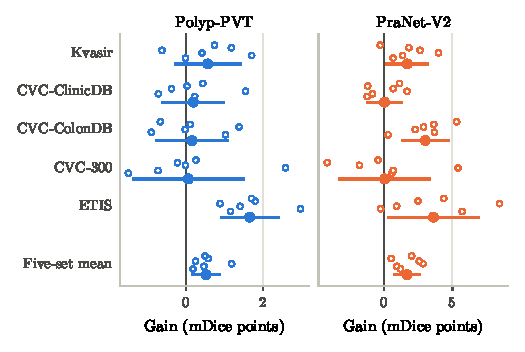
\includegraphics[width=\columnwidth]{figures/fig_seeds.pdf}
\caption{Paired gains of FCT over vanilla in mDice points: one hollow marker per seed, and the mean
with its 95\% CI below them. Every seed gains on the five-set mean for Polyp-PVT and PraNet-V2 and five
of six for ASGNet; the largest gains are on ETIS and, for PraNet-V2, CVC-ColonDB.}
\label{fig:seeds}
\end{figure}

Without epoch selection, the gains remain positive on average but are less certain.
Fig.~\ref{fig:curves} shows the five-set mean of the
training-time evaluator after every epoch: the six-seed mean of FCT lies above that of vanilla after 81
of 99 epochs for Polyp-PVT, 28 of 29 for PraNet-V2 and 76 of 79 for ASGNet. Averaged over the last ten
epochs, without any selection, FCT gains $+0.42$ $[-0.03, 0.88]$, $+2.41$ $[1.40, 3.43]$ and $+0.21$
$[-0.59, 1.01]$ points on the five-set mean of the three networks, and $+1.52$ $[0.11, 2.93]$, $+3.71$
$[0.75, 6.68]$ and $+1.99$ $[-0.26, 4.24]$ points on ETIS (Appendix, Table~\ref{tab:selfree}). At the last
epoch alone, no five-set mean gain has a CI above zero: $+0.55$ $[-0.11, 1.22]$ for Polyp-PVT, $+0.49$
$[-1.17, 2.14]$ for PraNet-V2, whose curves peak early and decline, so that its last epoch is a poor
checkpoint for either arm, and $+0.13$ $[-0.91, 1.17]$ for ASGNet.

\begin{figure}[t]
\centering
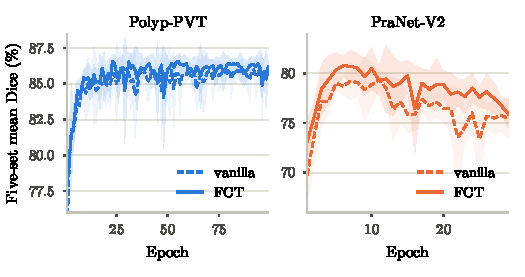
\includegraphics[width=\columnwidth]{figures/fig_curves.pdf}
\caption{Five-set mean Dice of the training-time evaluator after every epoch, without (dashed) and
with (solid) FCT; mean and SD over six seeds. FCT lies above vanilla through most of training. Every
ASGNet run, with or without FCT, drops briefly at epoch 62, so the drop comes from its recipe, not from
FCT.}
\label{fig:curves}
\end{figure}

\subsection{Six More Centres}
\label{sec:polypgen}

Of the five standard test sets, only ETIS comes from another centre than the training images
(Section~\ref{sec:setup}). PolypGen~\cite{ali2023polypgen} adds six more centres; we use its 1,411 single-frame images with a
polyp, none of which took part in training or in selecting a checkpoint. We fixed the analysis before
scoring any map: the primary result is the mDice pooled over the six centres, every image counted once,
over all six seeds, and each centre is a secondary result. So far, PolypGen maps exist only for the
confidence-graded weight, row (h) of Table~\ref{tab:rules}, and not yet for FCT. This label-aware
variant raises the pooled mDice of Polyp-PVT from 82.14\% to 82.98\%, by 0.84 points $[0.59, 1.09]$, on
all six seeds, and its gain has a CI above zero on four of the six centres (Table~\ref{tab:polypgen});
an exact permutation test over the 924 splits of the twelve runs gives $p=0.002$ for the pooled gain.
\pend{FCT's checkpoints will be scored with the same analysis.}

%% Generated by make_tables_extra.py; do not edit by hand.
\begin{table}[t]
\centering
\footnotesize
\setlength{\tabcolsep}{3pt}
\begin{threeparttable}
\caption{Six more centres (PolypGen): mDice (\%) of vanilla Polyp-PVT and of its confidence-graded variant, row (h) of Table~\ref{tab:rules}, mean $\pm$ SD over six seeds. Bold: gains whose 95\% CI excludes zero.}
\label{tab:polypgen}
\begin{tabular}{@{}l c c c c c@{}}
\toprule
Centre & Images & Vanilla & Variant (h) & Gain [95\% CI] & Seeds \\
\midrule
\enspace C1 & 251 & 86.65$\,\pm\,$0.42 & 87.94$\,\pm\,$0.55 & \textbf{+1.29 [0.71, 1.86]} & 6/6 \\
\enspace C2 & 270 & 84.60$\,\pm\,$0.47 & 84.31$\,\pm\,$0.64 & $-$0.28 [$-$1.27, 0.70] & 2/6 \\
\enspace C3 & 455 & 89.93$\,\pm\,$0.24 & 90.46$\,\pm\,$0.20 & \textbf{+0.53 [0.25, 0.81]} & 6/6 \\
\enspace C4 & 146 & 68.33$\,\pm\,$0.99 & 69.23$\,\pm\,$1.47 & +0.90 [$-$1.63, 3.44] & 4/6 \\
\enspace C5 & 206 & 65.71$\,\pm\,$1.65 & 67.92$\,\pm\,$1.25 & \textbf{+2.21 [0.38, 4.04]} & 5/6 \\
\enspace C6 & 83 & 82.88$\,\pm\,$0.29 & 84.23$\,\pm\,$0.45 & \textbf{+1.35 [1.04, 1.65]} & 6/6 \\
\midrule
Pooled & 1411 & 82.14$\,\pm\,$0.18 & 82.98$\,\pm\,$0.21 & \textbf{+0.84 [0.59, 1.09]} & 6/6 \\
\bottomrule
\end{tabular}
\begin{tablenotes}[flushleft]
\footnotesize
\item Single-frame images with a polyp; none was used in training or in selecting a checkpoint. Pooled: every image of the six centres counted once, the primary result of an analysis fixed before scoring. FCT itself: \pend{pending}.
\end{tablenotes}
\end{threeparttable}
\end{table}


\subsection{Flip Consistency}
\label{sec:flip}

FCT makes both networks more flip-consistent on every test set (Table~\ref{tab:flipgap}). It lowers the
five-set mean flip gap from 12.5\% to 7.5\% for Polyp-PVT and from 15.6\% to 10.2\% for PraNet-V2, and
the flip gap on the training images by 84\% and 76\%. The reduction holds on every seed and in every
row of the table. Two observations qualify it. First, flip consistency is not accuracy: the largest
reduction on a test set, 70\% for Polyp-PVT on CVC-ClinicDB, comes with almost no change in Dice, and CVC-ColonDB and
ETIS remain the least consistent sets after FCT. Second, training on flipped images lowers the flip
gap by itself. In preliminary single runs of Polyp-PVT, the multi-view supervision of row~(b) of
Table~\ref{tab:rules}, without the consistency term, reached a five-set flip gap of 8.2\%, and the official random flip and
rotation augmentation reached 6.8\%, below that of FCT; yet the five-set mean Dice of the latter,
85.75\%, was below that of every vanilla seed. A lower flip gap alone therefore does not explain the gains of FCT, and we
read it as a symptom that the views are tied together, not as the cause of the gains.

%% Generated by make_tables_extra.py; do not edit by hand.
\begin{table}[t]
\centering
\footnotesize
\setlength{\tabcolsep}{3.6pt}
\begin{threeparttable}
\caption{Flip gap (\%) of the predicted masks without and with FCT on each test set and on the training images, and its relative change. Means over six seeds; lower is better.}
\label{tab:flipgap}
\begin{tabular}{@{}l rrr rrr@{}}
\toprule
& \multicolumn{3}{c}{Polyp-PVT} & \multicolumn{3}{c}{PraNet-V2} \\
\cmidrule(lr){2-4} \cmidrule(l){5-7}
Images & Vanilla & FCT & Change & Vanilla & FCT & Change \\
\midrule
\multicolumn{7}{@{}l}{\textit{Seen}} \\
\enspace Kvasir & 6.3 & 4.1 & $-$35\% & 8.8 & 5.1 & $-$42\% \\
\enspace CVC-ClinicDB & 12.4 & 3.7 & $-$70\% & 13.1 & 5.9 & $-$55\% \\
\addlinespace[2pt]
\multicolumn{7}{@{}l}{\textit{Unseen}} \\
\enspace CVC-ColonDB & 16.9 & 11.3 & $-$33\% & 20.4 & 14.8 & $-$27\% \\
\enspace CVC-300 & 9.1 & 5.1 & $-$43\% & 9.8 & 6.2 & $-$37\% \\
\enspace ETIS & 17.8 & 13.2 & $-$26\% & 25.8 & 19.2 & $-$26\% \\
\midrule
Five-set mean & 12.5 & 7.5 & $-$40\% & 15.6 & 10.2 & $-$34\% \\
Training images & 6.3 & 1.0 & $-$84\% & 8.5 & 2.0 & $-$76\% \\
\bottomrule
\end{tabular}
\begin{tablenotes}[flushleft]
\footnotesize
\item Flip gap: one minus the Dice overlap of the binary masks predicted for an image and for its flipped copy, flipped back, averaged over horizontal and vertical flips and over images. FCT lowers it on every seed, in every row.
\end{tablenotes}
\end{threeparttable}
\end{table}


\subsection{Where Do the Gains Come From?}
\label{sec:where}

For PraNet-V2, the gains on the unseen sets are spread over many images: on ETIS, the 176 images
outside the ten largest gains and the ten largest losses contribute 2.94 of its 3.61 points. For
Polyp-PVT, they are more concentrated: on ETIS, the ten images with the largest gains contribute 1.78
points, more than the net gain of 1.65, and the other 176 images contribute 0.79.
Table~\ref{tab:errors} breaks the errors down at a threshold of 0.5 on the per-image min-max-normalized
maps. The two networks gain in different ways. PraNet-V2 fails less
often: the number of images with a Dice below 0.1 falls from 31.8 to 25.0 per run on ETIS and from 56.5
to 47.5 on CVC-ColonDB. Polyp-PVT fails about as often with FCT as without, 10.3 and 10.5 images per run
on ETIS; it gains instead by predicting less false-positive area, 1.31 instead of 1.52 times the polyp
area. In two cases, small polyps carry much of the gain:
the quarter of images with the smallest polyps gains 5.46 points on ETIS for Polyp-PVT and 6.16 points
on CVC-ColonDB for PraNet-V2. The pattern is not general: on ETIS, the smallest polyps gain 2.70 points
for PraNet-V2 and the next quarter 6.05, and on CVC-300 the smallest polyps lose with both networks. These
breakdowns are descriptive, and with four size groups per set and network, some differences are
expected by chance.

%% Generated by make_tables_extra.py; do not edit by hand.
\begin{table}[t]
\centering
\footnotesize
\setlength{\tabcolsep}{1.9pt}
\begin{threeparttable}
\caption{Where the gains come from on the unseen test sets, vanilla $\to$ FCT: failures, missed and false-positive area, and the gain on the smallest polyps. Means over six seeds.}
\label{tab:errors}
\begin{tabular}{@{}l c c c c c@{}}
\toprule
Test set & Gain & Failures & Missed area & False-pos.\ area & Smallest \\
\midrule
\multicolumn{6}{@{}l}{\textit{Polyp-PVT}} \\
\enspace CVC-ColonDB & +0.15 & 15.0 $\to$ 15.3 & 0.18 $\to$ 0.16 & 0.66 $\to$ 0.73 & $-$1.75 \\
\enspace CVC-300 & +0.06 & 0.2 $\to$ 0.0 & 0.06 $\to$ 0.06 & 0.23 $\to$ 0.27 & $-$2.38 \\
\enspace ETIS & +1.65 & 10.5 $\to$ 10.3 & 0.12 $\to$ 0.11 & 1.52 $\to$ 1.31 & +5.46 \\
\addlinespace[2pt]
\multicolumn{6}{@{}l}{\textit{PraNet-V2}} \\
\enspace CVC-ColonDB & +3.01 & 56.5 $\to$ 47.5 & 0.27 $\to$ 0.25 & 0.33 $\to$ 0.26 & +6.16 \\
\enspace CVC-300 & +0.04 & 0.2 $\to$ 0.0 & 0.05 $\to$ 0.06 & 0.25 $\to$ 0.23 & $-$1.85 \\
\enspace ETIS & +3.61 & 31.8 $\to$ 25.0 & 0.26 $\to$ 0.22 & 0.82 $\to$ 0.86 & +2.70 \\
\bottomrule
\end{tabular}
\begin{tablenotes}[flushleft]
\footnotesize
\item Gain: mDice points. Failures: images per run with Dice below 0.1 for the mask thresholded at 0.5 after per-image min-max normalization. Missed and false-positive area: at the same threshold, as fractions of the polyp area. Smallest: mDice gain on the quarter of the set with the smallest polyps.
\end{tablenotes}
\end{threeparttable}
\end{table}


Fig.~\ref{fig:qual} shows examples. Without FCT, PraNet-V2 misses the polyp in rows 1, 2 and 4, and
Polyp-PVT adds spurious regions in rows 1--3; with FCT, both predictions concentrate on the polyp. The last row shows the image on which FCT loses most: with FCT, Polyp-PVT adds a false region,
and PraNet-V2 misses the polyp.

\begin{figure*}[t]
\centering
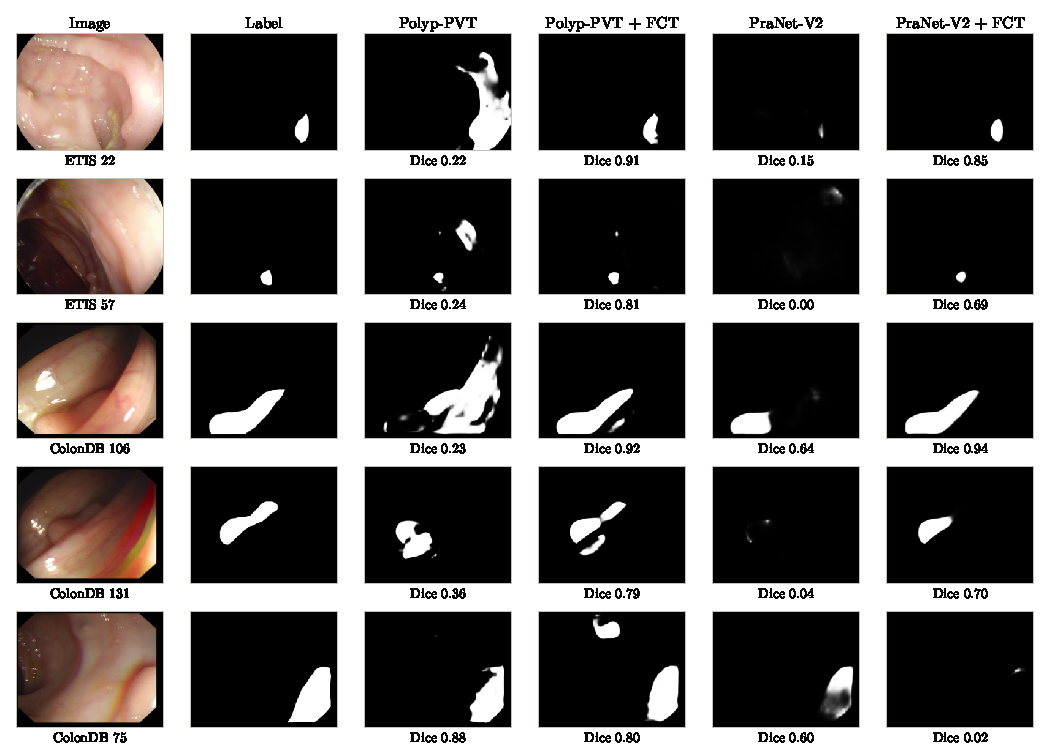
\includegraphics[width=0.94\textwidth]{figures/fig_qual.pdf}
\caption{Examples from the unseen sets: image, label, and the maps predicted by each network without
and with FCT (seed 1), each with its mDice. Rows 1--4: four of the twelve unseen-set images with the
largest gains, averaged over six seeds and both networks. Row 5: the image with the largest loss.}
\label{fig:qual}
\end{figure*}

\subsection{Ablation Studies}
\label{sec:ablation}

\textit{Loss terms.} The FCT loss has three parts: the multi-view supervision of Eq.~\eqref{eq:sup}, the
consistency term of Eqs.~\eqref{eq:flippull} and~\eqref{eq:uppull}, and the label-aware weights of
Eq.~\eqref{eq:weight}. Table~\ref{tab:rules} dissects them on Polyp-PVT, against the same vanilla runs
throughout. Row (b) keeps only the multi-view supervision. It is also the flip-augmentation control,
since it trains on exactly the views that FCT uses, with the same supervision. Rows (c)--(e) add the
consistency term on the upright view, on the flipped views, and on both, which is FCT, so their
differences from row (b) are the effect of the consistency term. Rows (f) and (g) change only the
weights of FCT, to unweighted consistency and to the lag gate without its margin. We fixed the protocol
before seeing these rows: rows (b) and (c) are trained with six seeds, and rows (f) and (g) with three
seeds first, extended to six only if they land near FCT. \pend{Row (c) is being repeated after a failed
run; rows (f) and (g) landed near FCT and are being extended to six seeds.} With six seeds, the paired
CI of the difference between two variants spans about $\pm0.4$ to $\pm0.7$ points on the five-set
mean, and with three seeds about 2.4 times more, so small differences between variants are not
resolved.

%% Generated by make_tables_extra.py; do not edit by hand.
\begin{table*}[t]
\centering
\footnotesize
\setlength{\tabcolsep}{2.6pt}
\begin{threeparttable}
\caption{Component dissection of FCT on Polyp-PVT: paired mDice gains (points, 95\% CI), the effect of each component, test sets improved, flip gap and gradient alignment. Bold: CIs that exclude zero.}
\label{tab:rules}
\begin{tabular}{@{}l c c c c c c c c c@{}}
\toprule
Variant & Views & Flip pulls & Upright pull & Mean gain & ETIS gain & Component effect & Sets & Flip gap (\%) & Cosine \\
\midrule
\multicolumn{10}{@{}l}{\textit{Building FCT on the three supervised views}} \\
(a) Vanilla & -- & -- & -- & -- & -- & -- & -- & 12.5 & -- \\
(b) Three views & \checkmark & -- & -- & \pend{pending} & \pend{pending} & -- & \pend{--} & \pend{--} & \pend{--} \\
(c) + upright pull & \checkmark & -- & \checkmark & \pend{pending} & \pend{pending} & \pend{pending} & \pend{--} & \pend{--} & \pend{--} \\
(d) + flip pulls & \checkmark & Eq.~\eqref{eq:weight} & -- & +0.47 [$-$0.02, 0.96] & \textbf{+1.97 [1.06, 2.87]} & \pend{pending} & 4/5 & 7.5 & 0.53 \\
(e) + both (FCT) & \checkmark & Eq.~\eqref{eq:weight} & \checkmark & \textbf{+0.52 [0.15, 0.90]} & \textbf{+1.65 [0.88, 2.42]} & \pend{pending} & 5/5 & 7.5 & 0.53 \\
\addlinespace[2pt]
\multicolumn{10}{@{}l}{\textit{Changing the weight function of FCT}} \\
(f) FCT, $w=1$ (3 seeds) & \checkmark & $w=1$ & \checkmark & \pend{pending} & \pend{pending} & \pend{pending} & \pend{--} & \pend{--} & \pend{--} \\
(g) FCT, lag only (3 seeds) & \checkmark & lag only & \checkmark & \pend{pending} & \pend{pending} & \pend{pending} & \pend{--} & \pend{--} & \pend{--} \\
\addlinespace[2pt]
\multicolumn{10}{@{}l}{\textit{Another label-aware weight, without the upright pull}} \\
(h) Graded weight & \checkmark & graded & -- & \textbf{+0.40 [0.13, 0.68]} & \textbf{+1.56 [0.53, 2.60]} & +0.06 [$-$0.60, 0.73] & 3/5 & 7.7 & 0.26 \\
\bottomrule
\end{tabular}
\begin{tablenotes}[flushleft]
\footnotesize
\item Six seeds unless the row says otherwise. Mean and ETIS gain: over vanilla with the same seeds. Component effect, on the five-set mean, paired by seed: for rows (c)--(e), the row minus row (b), so the effect of the pulls added to the three views; for rows (f) and (g), FCT minus the row, the effect of FCT\textquotesingle s weight function; for row (h), row (d) minus row (h). Sets: test sets, of five, with a positive mean gain. Cosine: between the gradient of the flip pulls and that of the rest of the objective, measured every 50 batches and averaged over training and seeds; for row (e), the rest includes the upright pull. Lag only: $w=1$ where the flipped view lags and $0$ where it leads ($a\to\infty$). Graded: the confidence-graded weight of Section~\ref{sec:ablation}.
\end{tablenotes}
\end{threeparttable}
\end{table*}


The multi-view supervision gives most of the gain on ETIS. On its own, row (b) raises ETIS by 1.48
points $[0.32, 2.65]$ on five of six seeds, against 1.65 points for FCT, and the five-set mean by 0.37
points $[-0.01, 0.74]$. This gain is not that of random flip augmentation: ASGNet already trains with
random flips, and FCT still raises its ETIS score by 1.69 points (Table~\ref{tab:main_asgnet}). The consistency term and its weights complete the loss: FCT is the only
variant that improves all five sets on average. The multi-view supervision alone lowers CVC-ClinicDB
by 0.48 points, and FCT recovers it, although this difference is borderline, $+0.66$ $[-0.01, 1.34]$.
The consistency term's own effect on the five-set mean, row (e) minus row (b), is $+0.16$
$[-0.30, 0.62]$ points, and the weight functions are within seed variation of one another: FCT minus
rows (f) and (g) is $+0.29$ $[-0.87, 1.45]$ and $+0.29$ $[-1.65, 2.23]$ points on three seeds, and
row (d) minus row (h) is $+0.06$ $[-0.60, 0.73]$. Row (h) uses the confidence-graded weight sketched in
Section~\ref{sec:relation}, which keeps a weight of 1 where the upright view is correct, raises it to
$1+p^{o}$ on missed polyp pixels and lowers it to $1-p^{o}$ on false-positive pixels.

The weights shape the gradient of the consistency term, as Eq.~\eqref{eq:weights} predicts. With the
lag-based weights of rows (d), (e) and (g), the gradient of the term on the flipped views has a cosine
of 0.53 to 0.56 with the gradient of the rest of the loss, and between 0.47 and 0.56 on every seed.
Without weights, row (f), it falls to 0.23, and with the confidence-graded weight, row (h), to 0.26;
these two stay between 0.18 and 0.33 on every seed (Fig.~\ref{fig:cos}). Unweighted and
confidence-graded terms keep full weight on leading flipped views, whose pixel weights in
Eq.~\eqref{eq:weights} are negative, so part of their gradient points away from the label. Leading
pixels are common: in the runs where we logged them, Polyp-PVT with $a<2$ and PraNet-V2, a flipped view
leads the upright view on about 44\% of its pixels at the end of training, although this is a share of
pixels, not of the gradient. The ratio of the two gradients' norms follows the same order: 0.07 to 0.08
with lag-based weights, against 0.11 without weights and 0.12 with the graded weight.

\begin{figure}[t]
\centering
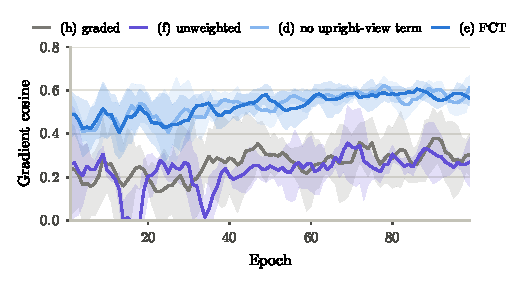
\includegraphics[width=\columnwidth]{figures/fig_cos.pdf}
\caption{Cosine between the gradient of the consistency term on the flipped views and that of the rest
of the loss during training of Polyp-PVT, for rows (d), (e), (f) and (h) of Table~\ref{tab:rules};
per-epoch means, smoothed over five epochs, with the SD over seeds. The lag-based weights double the
alignment of the consistency gradient with the rest of the loss.}
\label{fig:cos}
\end{figure}

\textit{Constant $a$.} The results are insensitive to $a$, so the constant needs no tuning
(Table~\ref{tab:sweep}; row (g) of Table~\ref{tab:rules} adds the limit $a\to\infty$, which keeps only
the lagging terms). Every value in $\{0.5, 1, 1.5, 2\}$ improves ETIS by 1.6 to 2.1 points, and none
differs significantly from $a=2$ on the five-set mean. The value $a=2$ is the only one that improves all
five sets on average, but this distinction is within seed variation. These runs do not fully explain
the insensitivity. The case that $a=2$ removes, a flipped view that leads a wrong upright view, is rare: it
arises on only 0.16\% of the pixels at the end of training (Polyp-PVT, $a<2$) and on 0.24\% (PraNet-V2).
But $a$ also scales the term on the far more frequent leading pixels with a correct upright view, and
this change, too, leaves Dice unchanged within seed variation.

%% Generated by make_tables_extra.py; do not edit by hand.
\begin{table}[t]
\centering
\footnotesize
\setlength{\tabcolsep}{2.2pt}
\begin{threeparttable}
\caption{Sensitivity to the constant $a$ of Eq.~\eqref{eq:weight} on Polyp-PVT: paired mDice gains over vanilla and over $a=2$ (points, six seeds, 95\% CI). Bold: CIs that exclude zero.}
\label{tab:sweep}
\begin{tabular}{@{}l c c c c@{}}
\toprule
$a$ & Mean gain & ETIS gain & Sets & $a=2$ minus row \\
\midrule
0.5 & \textbf{+0.51 [0.30, 0.73]} & \textbf{+2.15 [1.37, 2.92]} & 3/5 & +0.01 [$-$0.47, 0.49] \\
1 & +0.33 [$-$0.02, 0.67] & \textbf{+1.58 [0.40, 2.77]} & 3/5 & +0.19 [$-$0.26, 0.65] \\
1.5 & \textbf{+0.36 [0.02, 0.71]} & \textbf{+1.83 [0.83, 2.82]} & 3/5 & +0.16 [$-$0.24, 0.56] \\
2 (FCT) & \textbf{+0.52 [0.15, 0.90]} & \textbf{+1.65 [0.88, 2.42]} & 5/5 & -- \\
\bottomrule
\end{tabular}
\begin{tablenotes}[flushleft]
\footnotesize
\item Gains over vanilla on the five-set mean and on ETIS. Sets: test sets, of five, with a positive mean gain. Last column: paired difference on the five-set mean between $a=2$ and the row.
\end{tablenotes}
\end{threeparttable}
\end{table}


\subsection{Cost}
\label{sec:cost}

FCT multiplies the training time per epoch by 3.6 for Polyp-PVT, 3.3 for PraNet-V2 and 3.7 for ASGNet
(Table~\ref{tab:cost}). This matches its five forward and three backward passes for each image and input scale,
which cost $11/3\approx3.7$ times a single view if a backward pass costs twice a forward pass. Without
the term on the upright view, the two passes without gradient are not needed, and the measured factor
drops to 3.0. Inference
is unchanged: the trained network is the host network, applied once to the upright image.

%% Generated by make_tables_extra.py; do not edit by hand.
\begin{table}[t]
\centering
\footnotesize
\begin{threeparttable}
\caption{Cost of FCT: training time per epoch (minutes, median over six seeds) and inference cost.}
\label{tab:cost}
\begin{tabular}{@{}l c c c c@{}}
\toprule
Network & Vanilla & FCT & Ratio & Inference \\
\midrule
Polyp-PVT & 0.56 & 2.01 & 3.6$\times$ & unchanged \\
PraNet-V2 & 0.93 & 3.11 & 3.3$\times$ & unchanged \\
ASGNet & 1.01 & 3.70 & 3.7$\times$ & unchanged \\
Polyp-PVT, no upright-view term & 0.56 & 1.67 & 3.0$\times$ & unchanged \\
\bottomrule
\end{tabular}
\begin{tablenotes}[flushleft]
\footnotesize
\item Training time excludes the per-epoch evaluation. One \pend{[GPU model]} GPU per run. No upright-view term: row (d) of Table~\ref{tab:rules}. Inference: the same network, applied once to the upright image.
\end{tablenotes}
\end{threeparttable}
\end{table}

